% Options for packages loaded elsewhere
\PassOptionsToPackage{unicode}{hyperref}
\PassOptionsToPackage{hyphens}{url}
\PassOptionsToPackage{dvipsnames,svgnames,x11names}{xcolor}
%
\documentclass[preview]{article}

\usepackage{floatrow}
\DeclareFloatFont{small}{\small}% "scriptsize" is defined by floatrow, "tiny" not
\floatsetup[table]{font=small}

\usepackage[table]{xcolor}
\usepackage{multirow}
\usepackage{makecell}
\usepackage{array}

\usepackage{amsmath,amssymb}
\usepackage{algorithm}
\usepackage{algpseudocode}
\usepackage{iftex}
\input{preamble.tex}
\hypersetup{
  pdftitle={Group polarization replications may be marred by high false discovery rates},
  colorlinks=true,
  linkcolor={blue},
  filecolor={Maroon},
  citecolor={Blue},
  urlcolor={Blue}}


\newcommand{\mupre}{\mu_\mathrm{pre}}
\newcommand{\mupost}{\mu_\mathrm{post}}

\newcommand{\sigmapre}{\sigma_\mathrm{pre}}
\newcommand{\sigmapost}{\sigma_\mathrm{post}}

\newcommand{\thetafit}{\theta^\mathrm{fit}}

\newcommand{\fdr}{\mathrm{FDR}}

\newcommand{\meanobs}{\bar{o}}
\newcommand{\meanobsemp}{\bar{\mathbf{o}}}
\newcommand{\meanobst}{\meanobs_t}
\newcommand{\meanobsjt}{\meanobs_{j,t}}

\newcommand{\meanobspre}{\meanobs_\mathrm{pre}}
\newcommand{\meanobspost}{\meanobs_\mathrm{post}}
\newcommand{\tpre}{t_\mathrm{pre}}
\newcommand{\tpost}{t_\mathrm{post}}

\definecolor{myorange}{RGB}{240, 96, 0}
\newcommand{\mt}[1]{{\textcolor{myorange} {({\tiny MT:} #1)}}}

\usepackage{authblk}
\usepackage{etoolbox}
\usepackage{wrapfig}
\makeatletter
% \title{If the Null Fits, You Must Omit: Ubiquitous False Detections of Group Polarization}
\title{If the Null Fits, You Must Omit: Measurement Artifacts Undermine Group Polarization Replications}
\makeatother
\author[1,*]{{Matthew A.~Turner}}
\affil[1]{\small Environmental Social Sciences, Stanford Doerr School of Sustainability, Stanford University}

\author[2,3]{{Paul E.~Smaldino}}
\affil[2]{\small Cognitive and Information Sciences, University of California, Merced}
\affil[3]{\small Santa Fe Institute} 
% \vspace{2em}
\affil[*]{\small Correspondence: \href{mailto:maturner@stanford.edu}{maturner@stanford.edu}}

\date{\today}
\begin{document}
\maketitle

\renewcommand*\contentsname{Table of contents}
{
\hypersetup{linkcolor=gray}
\setcounter{tocdepth}{2}
\tableofcontents
}

\begin{center} \noindent\rule{4cm}{0.4pt} \end{center}
% \clearpage

% \begin{quote}
% In our introductory social psychology course, 
% we have for many years used the [group polarization experimental paradigm] as
% a laboratory exercise. The exercise works beautifully, but one must be
% careful to forewarn a class that [group polarization] does not occur with every 
% group\ldots and that the effect is not large. 
% \par\raggedleft(Brown, 1986, p.\cite[p. 205]{Brown1986})
% \end{quote}

% \begin{quote}
%   The good thing about science is that it's true, whether or not you believe
%   it. (Neil de Grasse Tyson slogan circa 2018)
% \end{quote}


% \subsection*{Abstract}\label{abstract}
\addcontentsline{toc}{subsection}{Abstract}

\emph{Group polarization} is the name for a form of consensus where
members of a like-minded group become, on average, more extreme in their
opinions after discussing a topic. Group polarization is important
because it may increase social and political tensions if moderates
become more extreme. Decades of studies have replicated detections of
group polarization, typically using an ordinal scale to measure
opinions. However, these studies did not account for ordinal
measurements, which can result in spurious detections of opinion change.
Lacking original data we can still calculate the probability that a
published detection of group polarization was spurious, i.e., to
calculate the \emph{false detection rate}. Across 54 group polarization
experimental conditions from ten representative journal articles, we
calculated false detection rates to be between 0.52 and 0.88, with a
median of 0.75, using a generative model of group polarization
experiments seeded with empirical data. We also use our model to develop
experimental designs that achieve an acceptable false discovery rate.
Much of group polarization research may be unreliable. This analysis can
help change that by enabling others to avoid this hidden pitfall. More
broadly this work demonstrates one important way that replication
success alone does not imply epistemic reliability.

\section{Introduction}\label{introduction}

\begin{quote}
In our introductory social psychology course, we have for many years
used the {[}group polarization experimental paradigm{]} as a laboratory
exercise. The exercise works beautifully, but one must be careful to
forewarn a class that {[}group polarization{]} does not occur with every
group\ldots and that the effect is not large (Brown 1986).
\end{quote}

\begin{quote}
One of the most robust findings in social psychology is that of attitude
polarization following discussion with like-minded others (Cooper,
Kelly, and Weaver 2001).
\end{quote}

If an extremist's opinion falls and it is measured with a Likert scale,
will it make a noise? The answer had better be yes if we want to
properly measure opinion change. Accurate measurements are critical for
developing rigorous and reliable methods to promote more stable,
sustainable, responsive, and efficient governments and institutions
(Mason 2018; Klein 2020). Unfortunately, social and behavioral
scientists have often used statistical methods that distort opinion
change when it's measured on an ordinal, Likert-style scale (e.g.~-3
indicates ``Strongly disagree'', +3 indicates ``Strongly agree'', and 0
is neutral) (Liddell and Kruschke 2018). This includes a phenomenon
called \emph{group polarization} that former Obama White House official
and law professor Cass Sunstein relied on to explain why ``people become
extremists'' and why ``political and cultural polarization'' is ``so
pervasive in America'', as the publisher summarizes (Sunstein 2009).
Sunstein suggests group polarization research provides a ``clue'' to
explaining how ``facism\ldots student radicalism\ldots Islamic
terrorism\ldots{[}t{]}he Rwandan genocide\ldots{[}e{]}thnic
Conflict\ldots acts of torture and humiliation by American soldiers at
Abu Ghraib'', and more (p.~1).

\begin{itemize}
\tightlist
\item
  We demonstrate here that there is a pervasive problem observed over
  decades of group polarization research where faulty statistical
  methods and incomplete reporting that should force the retraction of
  these studies from the canon. Effectively, then, empirical support for
  the theoretical concept \emph{group polarization} stops being so: the
  epistemic integrity of \emph{group polarization} is undermined with
  its empirical foundation losing mass.
\end{itemize}

We complement this critical analysis with a prescriptive analysis to
demonstrate that more appropriate statistical models do indeed lower the
false discovery rate by committing fewer false positive detections of
group polarization under a null model with shrinking opinion variance.
Recently, statistical best-practice is to use Bayesian models of
statistics, where social dynamics and opinion-reporting behaviors are
represented as causally-dependent probability distributions, where a
sample taken from one distribution (e.g., the opinion distribution of a
group in a group polarization experiment) acts as an input parameter to
another distribution (e.g., that represents the
individually-heterogeneous distortion of opinions when reported on an
ordinal scale). Our models follow current best practices in
psychometrics, social science, and Bayesian inference (Liddell and
Kruschke 2018; Kruschke 2015; McElreath 2020; Deffner et al. 2024), but
consolidate them in a new, useful way that enables the retroactive
discovery of null model parameters that generate spurious group
polarization, forcing published evidence for group polarization to be
classified as non-identifiable, and removed from evidence that can be
said to support group polarization.

Our methods can be turned on any data-driven social science analysis of
data where participants report a latent, subjective psychological
variable (mood, physiological state, etc.), and where various theories
supposedly battle it out to best represent the phenomenon of interest
via NHST performed on ordinal observations with weak, informal
theoretical models to motivate the studies. This may just be the first
of many bricks to fall since \emph{all 68} of the articles that
mentioned the word ``Likert'' and analyzed ordinal data used metric
models to detect latent psychological variable change across three
influential psychology journals, \emph{Psychological Science}, the
\emph{Journal of Experimental Psychology: General}, and the
\emph{Journal of Personality and Social Psychology} (Liddell and
Kruschke 2018).

This work is motivated by a core conviction that better thinking leads
to better science. Theoretical clarity, careful measurement, and
principled statistical modeling are not academic luxuries, but essential
tools for empirical science. Theoretical and statistical confusions in
the group polarization literature have lain dormant, undermining
measurements of opinion change in group polarization unbeknownst to
generations of researchers (Brown 1986).

\subsection{Identifiability and the Illusion of
Change}\label{identifiability-and-the-illusion-of-change}

\begin{itemize}
\tightlist
\item
  Many group polarization studies report opinion change based on
  pre/post differences, but assume a transparent mapping between
  observed scores and latent beliefs.
\item
  Yet ordinal opinion data can mask deeper structural ambiguities that
  invalidate these assumptions.
\item
  In what follows, we first describe the basic structure of group
  polarization experiments, then explain how ordinal measurement can
  lead to illusory shifts.
\item
  Finally, we introduce a null-consistency modeling procedure that
  operationalizes this insight, and show how it informs the credibility
  of reported effects.
\end{itemize}

\subsubsection{Experimental structure of group polarization
studies}\label{experimental-structure-of-group-polarization-studies}

\begin{itemize}
\tightlist
\item
  Most group polarization experiments follow a familiar structure:
  measure individual opinions, allow group discussion, then re-measure.
\item
  The central claim is that like-minded individuals become more extreme
  after deliberation.
\item
  Crucially, opinions are typically measured with Likert-style ordinal
  scales (e.g., from ``Strongly disagree'' to ``Strongly agree'').
\item
  Analyses often treat these as interval-scaled, calculating mean
  differences and testing for significance.
\end{itemize}

\subsubsection{The ordinal-continuous mismatch
problem}\label{the-ordinal-continuous-mismatch-problem}

\begin{itemize}
\tightlist
\item
  Ordinal scores do not have a fixed interval structure --- they
  represent ranked categories, not true distances.
\item
  A given change in score may reflect a shift in opinion, increased
  certainty, or both.
\item
  For example, if opinions become more tightly clustered (lower
  variance) post-deliberation, the group mean can appear to shift even
  when the latent mean remains unchanged.
\item
  This opens the door to \emph{null-consistent detections} --- apparent
  effects that emerge from measurement artifacts rather than real
  opinion movement.
\end{itemize}

\subsubsection{Description of the null-consistency modeling
procedure}\label{description-of-the-null-consistency-modeling-procedure}

\begin{itemize}
\tightlist
\item
  We formalize this concern using a generative model that holds the
  latent opinion mean constant while allowing variance to shrink.
\item
  The goal is to test whether an observed group polarization result
  could arise from such a stable-mean, shifting-variance process.
\item
  If this model can reproduce the pre/post measurement pattern, the
  observed result is non-diagnostic --- it is consistent with a null
  hypothesis of no true change.
\item
  This is a form of constructive falsification: it doesn't prove the
  effect is false, but shows it is not uniquely explained by change.
\end{itemize}

\subsubsection{Implications for statistical power and detection
credibility}\label{implications-for-statistical-power-and-detection-credibility}

\begin{itemize}
\tightlist
\item
  Even if an effect is real, detecting it reliably requires statistical
  power --- the ability to distinguish true shifts from noise or
  artifacts.
\item
  Studies using ordinal measures and small samples may be especially
  vulnerable to false positives under the null.
\item
  To assess this, we fit Bayesian ordered probit models to simulated
  data and estimate the power to detect effects of various sizes.
\end{itemize}

\subsubsection{Transition to empirical review and FDR
estimation}\label{transition-to-empirical-review-and-fdr-estimation}

\begin{itemize}
\tightlist
\item
  Having established a model-based definition of null-consistent
  detection, we now apply it to published group polarization
  experiments.
\item
  By combining this logic with simulations seeded from published data,
  we estimate false discovery rates across conditions.
\item
  This isn't a judgment about whether past detections were true. It's a
  demonstration of how to estimate false detection rates
  properly---using models that actually fit the structure of the data.
  We calculate FWER and FDR for the original study designs at three
  effect size levels---small, medium, and large---based on Cohen's
  guidelines (Cohen 1988, Ch. 2.2.3) and Bayesian methods from Liddell
  and Kruschke (Liddell and Kruschke 2018). The verdict is clear: even
  if these studies had used better models, most still wouldn't have had
  the power to rule out false positives. That makes replication a weak
  signal of reliability. If future group polarization studies want to
  produce meaningful result need stronger designs---and that starts with
  a clean break from outdated statistical habits.
\end{itemize}

The null-consistency procedure functions as a test of model
indistinguishability: it demonstrates that a reported group polarization
effect could plausibly arise from a stable-latent process combined with
changing opinion precision. This logic echoes foundational concerns in
causal inference, where two competing models---one causal, one not---can
imply the same observed data distribution and are therefore empirically
indistinguishable without further assumptions (Pearl 2000; Spirtes,
Glymour, and Scheines 2000). In such cases, inference from observation
to mechanism is invalid. Similarly, in psychometrics, it is well known
that different configurations of latent traits and response thresholds
can yield identical observed ordinal patterns, making the true structure
unidentifiable without additional constraints (Borsboom 2005). The
present approach does not attempt to estimate the probability of false
detection, but rather shows that under ordinal measurement, a null model
can reproduce the observed pattern---rendering the result non-diagnostic
of a true latent shift. This establishes a stringent standard: an effect
must not only be detected, but shown to be incompatible with plausible
null-generating mechanisms.


\input{intro.tex}

\section{Method}\label{method}

A group polarization replication is proven undecidable, and therefore not
truly a replication, if we can find a model of \emph{mere agreement} that
appears to be polarized under that replication's experimental design. If we
cannot find such a model, we cannot determine a replication to be
undecidable. Mere agreement in this model is a dynamic where agreement
increases within the group, but extremism does not—in other words, A
\emph{null-polarization distributions} is a set of two Gaussian
distributions: one representing the pre-discussion opinions of the group, and
the other representing the post-discussion opinions. Our
\emph{null-polarization distributions} represent the process of the group
finding \emph{mere agreement}, which is when the average group opinion is
constant over time, but opinion variance decreases to represent agreement
(or, equivalently, \emph{consensus}~\cite{DeGroot1974}).

Null-polarization  We thus model opinions at each time, $t=\mathrm{pre}$ and
$t=\mathrm{post}$, as random variables drawn from a normal distribution with
mean $\mu_t$ and standard deviation $\sigma_t$.  we drop the time 

The null-polarization distributions are represented by 

in a simple, general way—i.e., a decrease in opinion variance but a static
opinion mean—we represent . In the general group polarization hypothesis, the
group is assumed to start out mostly agreeing in principle (i.e., mostly all
agree or disagree) but to different extremes. After discussion

Showing a replication is undecidable is sufficient to undermine it. However,
it does not tell us what is the probability that a particular experimental
design produces false positives, due to clipping or any other problem. 

first develop a mathematical model of estimate the best-case scenario false
positive rate for each experimental design,


\subsection{Mathematical Model of Null-Polarization Measurement Artifacts}

Latent opinions are modeled as normally-distributed random variables.  
This is a simple, sufficiently general way to represent group-level changes
in opinions as encoded in the general hypothesis of group polarization, that
likeminded groups tend to become more extreme on average as they discuss.
For time, $t$, then, we represent each participant $i$'s opinion as 
\begin{equation} 
  \omega_{i,t} \sim \mathcal{N}(\mu_t, \sigma_t).
  \label{eq:opinionDistribution} 
\end{equation} 
\noindent 

Group-level opinion change, then, can be represented as a change in opinion
mean, opinion variance, or both. Group polarization occurs 
when a group's average opinion increases over time. When likeminded people
interact, they tend to come to agree more over time—they \emph{find consensus}. 
By definition this means opinion variance decreases, 
whether the average changes or not.

We can define a null-polarization model, then, as one where the group's
average opinion stays constant, but the variance decreases: $\sigmapost
\leq \sigmapre$. Since the mean opinion is constant we just call it 
$\mu = \mupre = \mupost$. For conciseness, we define a null-polarization
model as a 3-tuple, $\nu = (\mu, \sigmapre, \sigmapost)$. 

\begin{center}
\vspace{1.5em}
[ TABLE \ref{tab:latent-variables} ABOUT HERE ]
\vspace{1.5em}
\end{center}

\subsubsection{Simulated opinion measurements}

We simulate the collection of an \emph{ordinal distribution} of \emph{ordinal
observations}, as was performed in a prototypical group polarization experiment 
by integrating the latent opinion probability density function, $f(\omega)$,
over each bin's corresponding range of opinion values. For example, consider an
ordinal scale that runs from -3 (strongly disagree) to +3 (strongly agree)
(as used by \textcite{Moscovici1969}, for example).
the frequency with which the ``2'' bin is chosen is just the total
area underneath the probability density curve between 1.5 and 2.5.

Formally, the probability density function is
\begin{equation}
  f(\omega) = 
    \frac{1}{\sigma \sqrt{2 \pi}} e^{-\frac{(\omega - \mu)^2}{2 \sigma^2}}.
  \label{eq:normal_pdf}
\end{equation}
\noindent
To set up our measurement simulation, we will represent
oridnal bin values as $b_i$ with $i=1,\ldots,B$—i.e., there are $B$ bins. 
To create $B$ bins there must be $B+1$ \emph{thresholds} that define what
range of latent opinions correspond to which ordinal bin value. 

\begin{center}
  \vspace{1.5em}
  [ TABLE \ref{tab:experiment-parameters} ABOUT HERE ]
  \vspace{1.5em}
\end{center}

All bins have a width of 1 in latent opinion space, except for the two most
extreme bins at opposite ends of the sentiment spectrum—this works because
bin values are always separated by 1. All continuous latent opinion values
$\omega < b_1 + \frac{1}{2} = \theta_1$ get mapped to the ordinal measurement
value $b_1$—so, $b_1$'s lower threshold is $\theta_0 = -\infty$.  Similarly,
all opinions $\omega > b_B - 0.5 = \theta_B$ are reported as the maximum bin
value, $b_B$, with an effective upper bound of $\theta_{B+1} = +\infty$.  We
can define all thresholds compactly as \cite{Liddell2018}
\begin{equation}
\theta_j = \begin{cases}
  -\infty         & \text{ if } j=0 \\
  \infty          & \text{ if } j=B \\
  b_1 + \frac{j + 1}{2} & \text{ otherwise.}
\end{cases}
\label{eq:thresholds}
\end{equation}
\noindent

We model the measurement of ordinal opinions by calculating the probability
density function over bins, written
\begin{equation}
  f[b_i] = \int_{\theta_{i - 1}}^{\theta_i} f(\omega) d\omega~,
  \label{eq:measurement-math}
\end{equation}
\noindent
switching to square brackets for the argument to $f$ now to emphasize that 
bins are discrete. With this ordinal measurement model we can caluclate the 
mean opinion of the simulated measurements like so
\begin{equation}
  \bar{o}_t = \frac{1}{B} \sum_{b=b_1}^{b_B} b \cdot f_t[b].
\end{equation}
\noindent

\begin{center}
\vspace{1.5em}
[ FIGURE \ref{fig:distros} ABOUT HERE ]
\vspace{1.5em}
\end{center}

Group polarization is the difference between the post-deliberation mean
observed opinion and the pre-deliberation one, 
which we can write as 
\begin{equation}
  g = \bar{o}_\mathrm{post} - \bar{o}_\mathrm{pre}.
  \label{eq:group-polarization}
\end{equation}
\noindent

\begin{center}
\vspace{1.5em}
[ TABLE \ref{tab:simulated-observations} ABOUT HERE ]
\vspace{1.5em}
\end{center}


\subsection{Root-finding Algorithm to Find Null-Polarization Models with Artifacts}


\subsection{Corpus Analysis to Determine Undecidable Replications}

To analyze published replications we need to expand our notation to index
individual \emph{experiments} with replications, and from which 
different journal articles, track and analyze it, 


\subsection{Evaluating Grouop Polarization Experimental Designs}





\section{Analysis}\label{analysis}

We now present our determinations of whether published detections of group
polarization are plausibly spurious and calculate the best-case false detection
rate for each experimental design in the corpus. We found that 95\% of all
detections of group polarization are plausibly false, 54 out of 57. We estimate the
best-case median false detection rate to be 72\% for those 54 experimental
conditions. All but seven of the 54 designs were found to require a $d^* > 0.8$
for ``significant'' Cohen's $d$ to limit the family-wise error rate to 5\%.


\subsection{Nearly all group polarization detections are plausibly spurious}


% We used our formal distribution model of group polarization experiments
% to identify plausible latent simple consensus distributions that generate spurious
% group polarization in 
Of the remaining 57, we identified simple consensus $\nu$ that generate spurious
group polarization in 54 experimental conditions. In the other three, we did
identify $\nu$ that generate spurious group polarization, but the initial
simulated distributions were highly polarized. 
We rejected $\nu$ generated for
two spurious group polarization from Schkade, et al., (2010) because
the histogram plots of the observed opinion distributions are not
polarized~\cite[Figure 1, p. 234]{Schkade2010}. The other condition where we
found but rejected spurious group polarization $\nu$ was in a question 
about a ``bad teacher'' in Myers (1975)~\cite{Myers1975a}, where lower values
signify increasingly worse impressions of the teacher and higher values signify
increasingly good impressions. It is unlikely that a
``bad teacher'' would be rated as good in this case, so we excluded this 
from our analysis as well. This exclusion may be overly generous since Myers (1975)
did not provide details beyond mean values and opinion shifts, and the article was
published before open data practices. Our corpus had a total of 60 experimental conditions, but we excluded 3 out of 60 
that did not claim to be positive findings of group polarization.

- Address sigmas, note differences

\begin{figure}
  \centering
    \includegraphics[width=\textwidth]{Figures/3.1/latent-sd-cdf.png}
    \caption{\textbf{}}
  \label{fig:}
\end{figure}



\subsection{Half of experiments exceed a 70\% false discovery rate at ``medium'' significance}

We simulated trials from each experimental condition, $e$, by sampling and binning
pre- and post-deliberation latent opinions from distributions with parameters
identified with the $N\to\infty$ model as causing plausibly spurious group
polarization. For each $e$, we drew a number of samples equal to the number of
participants in the original experiments, $N_\mathrm{emp}$. To estimate family-wise
error and false detection rates, we fit an ordered probit model to the simulated
observations and obtained estimates of the group polarization effect size, $d$
(Equation~\ref{eq:cohens}). If the effect size was greater than a significance
value, $d > d^*$, then by definition there was a detection $D$ of group
polarization, even though there was no effect by design, written $\neg E$.  The
family-wise error rate is $\Pr(D|\neg E)$, calculated as the frequency with which $d
> d^*$ out of 1000 simulation trials. The false detection rate is the family-wise
error rate scaled using the base rate of effects and the statistical power
(Equation~\ref{eq:fdr}). We test three difference significance values, $d =
0.2,~0.5$ and $0.8$, corresponding to what Cohen prescribed to use for ``low'',
``medium'', and ``high'' significance. If not otherwise noted, we set the base
rate to be $b=0.1$ and the power $W = 0.8$ as metascience parameters to calculate 
the false discovery rate (Equation~\ref{eq:fdr}). Note that if the family-wise error
rate is low at $\alpha = 0.05$, the false discovery rate is $\fdr = 0.36$.

Different conditions yield different effect size distributions
(Figure~\ref{fig:effect_size_distros}), which 
determine the magnitude of error rates and difference between the error rates for low,
medium, and high significance values $d^*=0.2,0.5,0.8$ magnitude of error rates 
(Figure~\ref{fig:fwer_fdr_synthesis}B). 
Family-wise error rates varied from a minimum of one in ten for the
\texttt{Feminists-Experimental} condition from Myers (1975)~\cite{Myers1975a}
to a maximum of two in three for the \texttt{COSprings-CivilUnions} condition from
Schkade, Sunstein, and Hastie (2010)~\cite{Schkade2010} under medium
significance effect size $d^* = 0.5$ (Figure~\ref{fig:fwer_fdr_synthesis} and
Table~\ref{tab:quantiles}). The median family-wise error
rate is 0.28 for Krizan and Baron's (2007) experimental condition
\texttt{NoOutgroupScenario1}~\cite{Krizan2007}. This translated to a minimum
false detection rate of 0.52 for the Myers (1975) condition, a maximum false
detection rate of 0.88 for the Schkade, et al., (2010) condition, and a median false
detection rate of 0.75 for the Krizan and Baron (2007) condition. 

\begin{table}[ht]
  \caption{{\textbf{Quantiles for the two error-rate measures under different
  significance values.}}}
  \label{tab:quantiles}
  \centering
  % latex table generated in R 4.3.3 by xtable 1.8-4 package
% Tue Dec 31 16:29:18 2024
\begin{tabular}{lcccccc}
  \toprule
Measure & $d^*$ & Min & 20\%    & 50\%     & 80\%    & Max \\ 
  \midrule
   & 0.20 & 0.14 &  0.25  & 0.34   & 0.41  & 0.69 \\ 
  FWER, $\alpha$ & 0.50 & 0.07 &  0.16  & 0.23   & 0.30  & 0.60 \\ 
  & 0.80 & 0.03 &  0.10  & 0.15   & 0.21  & 0.46 \\ 
  \hline
  & 0.20 & 0.60 &  0.74  & 0.79   & 0.82  & 0.89 \\ 
  FDR  & 0.50 & 0.43 &  0.64  & 0.72   & 0.77  & 0.87 \\ 
  & 0.80 & 0.23 &  0.53  & 0.63   & 0.70  & 0.84 \\ 
   \bottomrule
\end{tabular}

\end{table}

In the conditions
with lower family-wise error rates, there were several conditions where using the low 
significance value $\alpha$ resulted in a much greater error rate than the medium or 
high significance values. In the ten conditions with the lowest $\alpha$ for 
$d^* = 0.5$, with $\alpha$ near 0.1, five of these conditions have $\alpha > 0.25$
when $d^* = 0.2$ corresponding to a small effect size. For low $\alpha$, the
difference in false detection rates for each $d^*$ value are more widely
distributed, following the distribution of $\alpha$, meaning that 
a modest increase in $d^*$ can have greater effects on the false discovery rate. In
the conditions above the 50th percentile, $\alpha$ approaches and exceeds one in
two, even when requiring ``high'' significance with $d^*=0.8$. With $d^* = 0.8$,
$\alpha$ approaches and exceeds one in four, with four near one in two. When 
requiring ``low'' signifance, 

Experimental designs within each study or article tend to share certain
characteristics, such as the number of bins in the ordinal measurement design
or the number of participants per condition. Therefore, the 
average false detection rate across experimental trials within a study
(Equation~\ref{eq:study_aggregate}) show that 

\begin{figure}

  \caption{\textbf{Family-wise error rates and false discovery rates across studies and experiments for
    low, medium, and high Cohen's $d$ significance.}}
  \label{fig:fwer_fdr_synthesis}

  \centering
  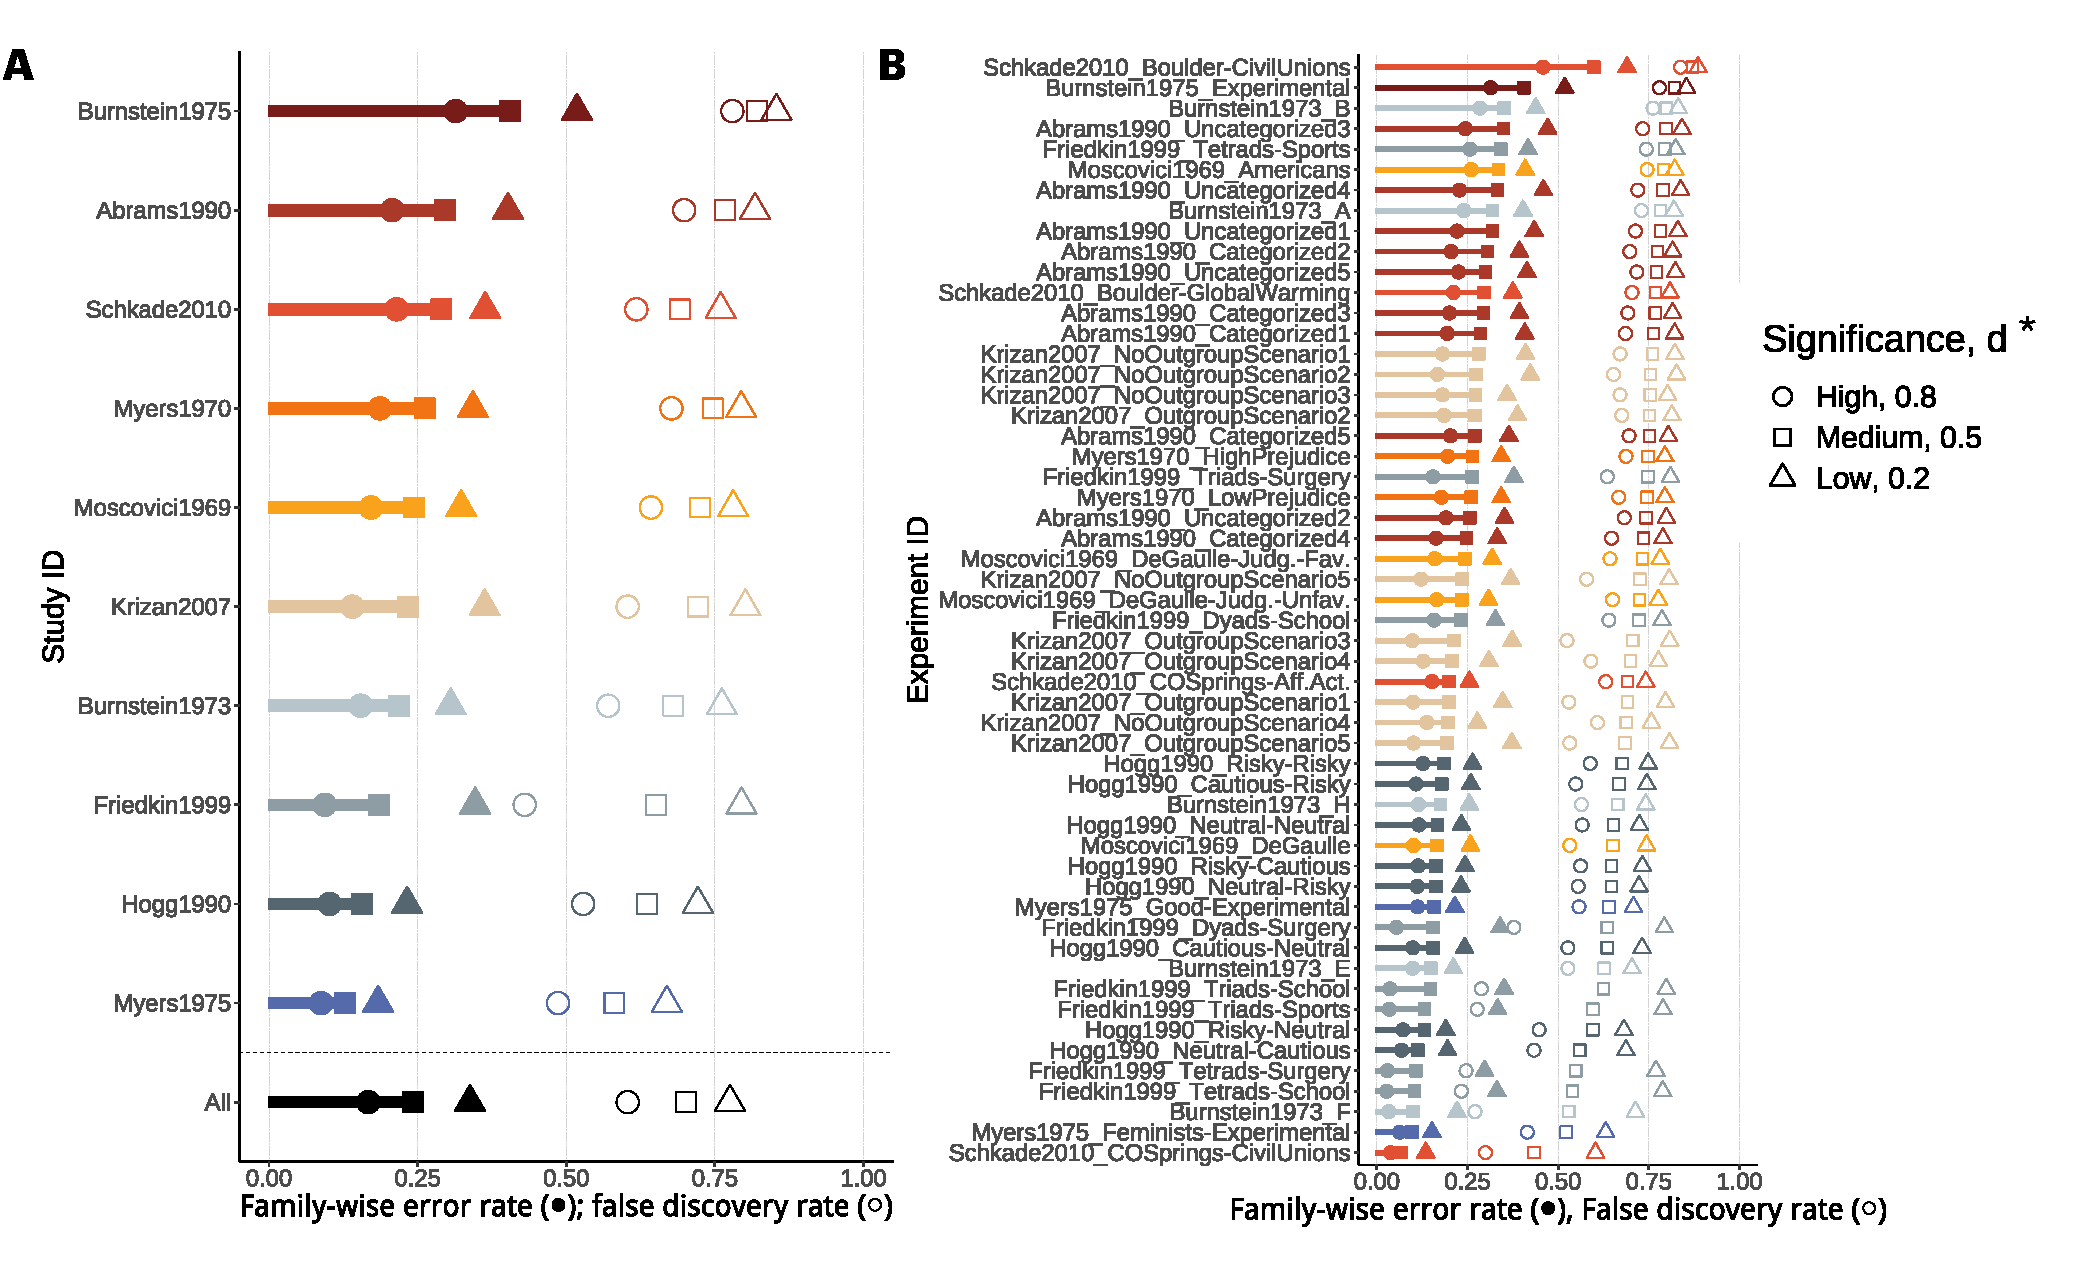
\includegraphics[width=1.1\textwidth]{Figures/Analysis/fwer_fdr_synthesis.pdf}
\end{figure} 

\begin{itemize}
  \item 
    Other $b$ and $W$ values in quantiles.
  \item
    Note that there were many ``significant'' results---in the wrong direction
    (Figure~\ref{fig:OrdinalBoxplot}).
\end{itemize}

\subsection{High significance values ($d^*$) often necessary for FWER of 0.05}

Our simulations can be used a different way, in this case to calculate what
significance value $d^*$ limits the family-wise error rate to the low value of
0.05. 
Solving the inverse problem of which $d^*$ achieves a low family-wise error rate,
which drives the false detection rate. Here we present our calculations to find
$d^*$ that achieve $\alpha(d^*) = 0.05$. 


\begin{figure}
  \caption{
    \textbf{Significance value, $d^*$, to limit family-wise error 
    rate of 0.05 for each identified study.} The Moscovici and Zavalloni (1969)
    ``Americans'' question would require the greatest $d^*$ to achieve $\alpha \leq
    0.05$, even though it does not have the highest error rates. This is because of
    larger outliers in simulated $d$ for this condition compared to others with
    greater error rates (Figure~\ref{fig:OrdinalBoxplot}).
  }
  \centering
    \includegraphics[width=0.75\textwidth]{Figures/Analysis/sigval_for_low_fwer.pdf}
  \label{fig:sigval_for_low_fwer}
\end{figure}



\section{Discussion}\label{discussion}

\mt{Restate results and importance and outline this section.}

Since there seems to be no selection pressure on false discovery rates,
experiment design for studying group polarization was free to evolve
randomly. Various choices for the number of bins and other instrumental
details may have then become entrenched in different communities defined by
common theoretical perspectives taken by researchers in those communities.
Therefore, when Isenberg (1986)~\cite{Isenberg1986} reports that his
meta-analysis found more support for the persuasive arguments theory than the 
social comparisons theory in the form of greater effect sizes. If this were
indeed the case, perhaps it is only because some researchers hypothesizing
persuasive arguments happened to use a measurement procedure produced more
frequent and extreme distortions of opinion measurements. Incentive
structures known to promote the ``evolution of bad science'' would select
for research that ignored sticky, time-consuming statistical problems in
favor of juicy titles and headlines for which practitioners have won several
professional awards. Specifically, the traditional bias
towards positive results, and against negative ones, could easily have
provided a cultural niche in which quick but faulty group polarization
statistical methods dominate slower, more rigorous ones.
Now that we are aware of the problem, there must be
intense selective pressure applied as soon and as widely as possible to 
avoid further ``replications'' that report spurious group polarization, or
any similar latent psychological dynamics. 

We provided tools that experimenters can use. While these tools are
potentially useful, they are still in the prototype phase that was
sufficient for a single researcher who was also the software developer. So,
a first step towards expanding the usefulness of the findings here is to 
improve the software usability and make the app widely available for
researchers in group polarization and beyond. Another step would be to go
beyond reactionary testing of the reliability of experimental designs, and
identify design principles that reduce the false detection rate without
needing to adjust the Cohen's $d$ (or whatever measure) 
used as a significance threshold. 

When we used the appropriate ordered probit Bayesian statistical model, it
still often failed to accurately identify mere agreement, instead detecting
group polarization.  The ordered probit model we used still likely
underestimates the variance in outcomes, which could require even larger
sample sizes. A more rigorous analysis would include additional sources of
variance that will likely further inflate the Type I error rate, $\alpha$,
and the false discovery rate~\cite{Yarkoni2022}. First and foremost, there is
variance within each experimental deliberation group; no group polarization
study accounts for this, instead treating participants in each experimental
condition as if they were one large group. Furthermore, survey data are known
to be noisy~\cite{Zaller1992}. People report opinions differently over time
for no apparent reason (i.e., opinions are \emph{unstable}).  Context
matters: the order in which a survey question is asked, and which question
framing is chosen among logically equivalent alternatives, can both
significantly influence participant responses. Finally, little is known about
the psychological process that converts latent opinions to reporting
behaviors (e.g., clicking a radio button corresponding to an opinion).  The
effect of accounting for these sources of variance must be understood to
estimate $\alpha$ (and power, $W$) for the design of the next generation of
group polarization experiments. 

A simple change in measurement procedure could fix the problem identified
here: center the post-discussion scale on each group’s own pre-discussion
mean. This removes the assumption that all groups share a common “neutral”
midpoint. The situation is like tossing a ball on a moving train: to the
passengers, the ball’s speed is the same in both directions, but to an
observer on the ground one throw appears faster and the other slower.
Likewise, when measurement is anchored to an external scale, simple agreement
within a group can appear as movement toward one pole. Re-centering the
measurement frame corrects this distortion. It acknowledges that opinion
change is relative to the observer’s reference frame—there is no fixed
background of neutrality against which all groups can be compared. This is,
in essence, the insight of Newtonian relativity: apparent motion depends on
the frame from which it is measured.

First we must note that there are even more, perhaps even graver problems
with group polarization research than I discussed so far: one of note is
opinion instability. Opinions are not generally stable—people seem to
construct their opinions based on several factors not directly related to
whatever underlying topic. Factors affecting reported opinions include the
language used to frame a prompt or question; the order of questions on a
multi-item survey; or simply when the question was asked (Kalton and Schuman,
1982; Zaller and Feldman, 1992; Zaller 1992). Failure to account for sources
of input variance in any experiment can lead to inflated effect sizes since
the input variance is missing from the posterior predictions during
statistical model fitting (Yarkoni, 2022). This further compounds the
theoretical confusions that fill the void when theories are never formalized
and grounded in a mathematical or computational model (Smaldino 2020; Turner
and Smaldino, 2022).

A second additional problem with group polarization research is that we literally cannot learn anything by comparing summary statistics obtained with incommensurate experimental designs—but this is exactly how group polarization research has tried to make progress. Comparing summary statistics only has explanatory power if datasets were generated under the same experimental designs—it seems this was never done or even considered in the group polarization literature. In order to compare studies, their datasets must be generated from commensurate experiments, meaning the studies must share the same predictive and statistical models and experimental design. Otherwise, such comparisons are meaningless, they literally tell us nothing, as shown by philosopher of science Nancy Cartwright in Chapter 5 of her book The Dappled World: A Study of the Boundaries of Science.


\subsection{Humble Hearts Promote Rigorous Science}

Cass Sunstein kicked off the 2000s by elevating group polarization to be a scientific law and advocating the application of group polarization research to serious real-world problems in two books (Sunstein, 2009; Sunstein, 2019) and two recent high-profile articles in Nature Human Behavior: one on the social foundations of pandemic preparedness (Van Bavel, et al., 2020) and one to “promote truth, autonomy, and democratic discourse online” (Lorenz-Spreen, Lewandowski, Sunstein, and Hertwig, 2020). Let us try to stop the spread of this bad science—and let us explore what must be done to achieve Dorian Cartwright’s vision of a rigorous science of group polarization he articulated fifty years ago.

To be practically useful, science must be rigorous. Rigorous science comes most naturally when scientists remain humble, especially when they serve at the pleasure of the public, the government, or other donors. Here’s another example from Burnstein and Vinokur (1973) that we can learn from—let’s try to avoid the sort of arrogance and haughtiness that seep from these acknowledgements they wrote on p. 123:

\begin{quote}
This research was supported by a Grant from the National Institute of Mental Health (MH-16950-03) and by a Guggenheim Foundation Fellowship awarded to the first author. We gratefully acknowledge the incisive, witty, and vinous commentary provided by colleagues at the University of Provence, in particular Robert Abelson, Claude Flament, and Jean-Pierre Poitou, as well as the spirited and intelligent efforts of Livia Mezrick and Irene Graczyk, who helped us carry out the study.
\end{quote}

Science is not glamorous—it takes guts and sacrifice to achieve the technical skills and discipline to sharpen one’s prose, methods, mathematics, and computer code to the point they can really cut reality at its joints, investigate different parts, then put it all back together with a message for others about how the world really works. These days, to do rigorous social science work one must wisely curate the best of the available social science by harmonizing cross-disciplinary jargon. But disincentives still exist against careful scholarship. Prizes and professorships go to those with the most numerous publications in the right journals—period.

Unpaid, anonymous reviewers are supposed to act as gatekeepers to catch problems like the ones I reviewed. But, journal article reviewers have little to gain from enforcing rigor—actually there is a lazy strategy that can pay off big for freeloaders. It’s easy to imagine a cultural norm evolving where reviewers save themselves time and energy by asking little of an author, in hopes that little will be demanded of them when the reviewer submits their next paper. This could result in a publication process that rewards the laziest and most willing to flood the zone and self-aggrandize.

\subsection{Conclusion}

Social science can use physics as a model discipline to transition from idiosyncratic and Balkanized to informative and united. Physics only changed the world because it is useful—it is useful only because it reliably predicts things. Physics became more useful as it became more united, finding shared representations for concepts developed independently—for example the science of optics was developed independently from the science of dynamics, but the physics of light is explained partly in analogy to a pendulum or spring—the mathematics of harmonic motion can be used to predict the motion of springs or pendulums—or why we see different colors of light through a prism. With careful, coordinated tweaks to group polarization experimental design and theoretical modeling, we will build a more rigorous theory of group polarization and its large-scale expression, echo chamber radicalization.

I expect that group polarization experiments, when properly constructed and analyzed, will help sustainability campaigns optimize their social influence campaigns. We can start by developing simpler experimental designs based on formal or computational models capable of predicting outcomes in an experiment. I have developed a model that could motivate an experimental design: I showed that if extremists are more stubborn, this is sufficient to cause group polarization when likeminded groups interact over time. There is even a free stubborn extremism parameter that could be fit to data to measure the relationship between stubbornness and extremism on different issues.

Group polarization research so far has mostly provided us with a checklist of what not to do. The alternative approach I outline builds on rock—the rock of rigor—and will supersede past group polarization research built on a thousand grains of inexact verbal speculation.



\printbibliography[title=References]

\appendix

\renewcommand{\thefigure}{A\arabic{figure}}

\setcounter{figure}{0}

\clearpage

%%%%%%%%%% Supplement %%%%%%%%%%
\pagebreak
\begin{center}
  \textbf{\Large \textsf{Group polarization replications may be marred by high false discovery rates (Supplementary Material)}}
\end{center}

%%%%%%%%%% Prefix a "S" to all equations, figures, tables and reset the counter %%%%%%%%%%
\setcounter{equation}{1}
\setcounter{figure}{0}
\setcounter{section}{0}
\setcounter{table}{0}
\setcounter{page}{1}
\makeatletter
\renewcommand{\theequation}{S\arabic{equation}}
\renewcommand{\thefigure}{S\arabic{figure}}
\renewcommand{\thetable}{S\arabic{table}}
\renewcommand{\thesection}{S\arabic{section}}
\renewcommand{\thepage}{S\arabic{page}}

\section{Analysis}

\begin{figure}
  \caption{Boxplot of Cohen's $d$ for the ordered probit model over 1000
    simulation trias for each experimental condition (y-axis in A and B). Each
    trial represents a possible outcome of a group polarization experiment where
    the true opinion shift is zero. The mean across trials is closer to 0 than
    in the metric case, but many simulated zero-shift experiments still result in
    an observed shift. This illustrates the weak statistical power of these group
    polarization experiments.}
  \label{fig:OrdinalBoxplot}
  \centering
    \includegraphics[width=1.0\textwidth]{Figures/Analysis/ordinal_cohens.pdf}
\end{figure}


\end{document}
